%% Digital Systems
%% Continuous System Equivalence
\def\FileDate{10/01/21}
\def\FileVersion{1.0}
% ----------------------------------------------------------------
% Notes pages *********************************************************
% ----------------------------------------------------------------

\begin{slide}
	\heading{Purpose of this Lecture}
	To describe the basic tools for the design of a control system to be implemented using a computer or microcomputer.

	\textbf{Contents}
	\begin{itemize}
		\item Typical architecture
		\item Relationship between $s$ and $z$
		\item Continuous design followed by Discretization
		\item Direct digital design
	\end{itemize}
\end{slide}

\section*{Typical Architecture of a Digital Control System}

\begin{slide}
	\heading{Typical Architecture}
	\begin{center}
	\resizebox{300pt}{!}{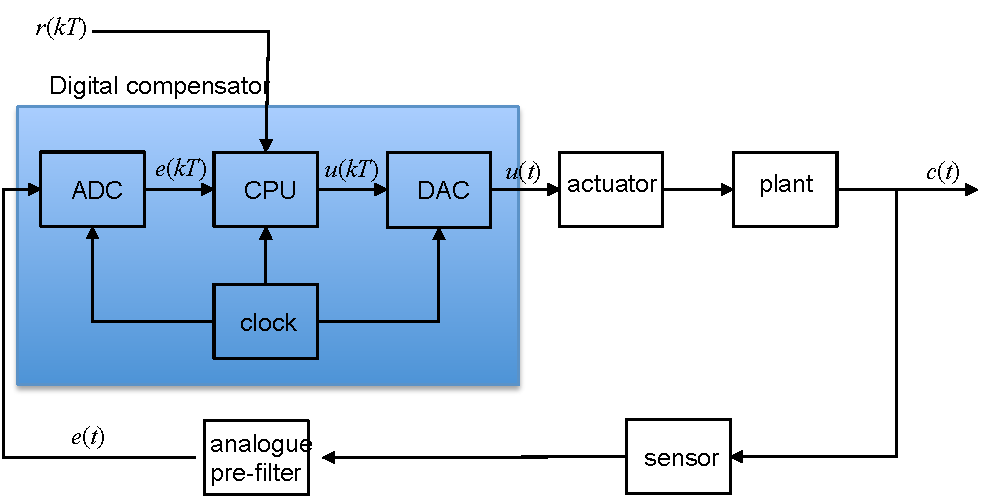
\includegraphics{pictures/digicon.pdf}}
\end{center}
\end{slide}

\section*{Relationship between $s$ and $z$}

We have already seen (SLIDE~2, lecture 11) that
\begin{equation}\label{eq:l12e1a}
	z=e^{sT}
\end{equation}
and
\begin{equation}\label{eq:l12e1b}
	s=\frac{1}{T}\ln z
\end{equation}
We can use Equation~\ref{eq:l12e1a} to define a mapping between the $s$ and $z$ planes as summarised in SLIDES~\ref{slide:l12s2} and \sref{slide:l12s3}.
\begin{slide}\label{slide:l12s2}
  \heading{Mapping between between $s$ and $z$}
  Since $z=e^{sT}$ we can define a `mapping' from the $s$-plane to the $z$-plane. Various properties of the $z$-plane follow.
\begin{itemize}
  \item s-plane stability boundary $s=j\omega$ maps to the unit circle $|z|=1$ in the z-plane.
  \item Maximum frequency is half the sampling frequency $\omega_s/2$ (a consequence of Nyquist's sampling theorem) and is mapped to the negative real axis in the z-plane.
\end{itemize}
For proofs, see the problems in the self-directed learning exercises.
\end{slide}

\begin{slide}\label{slide:l12s3}
  \heading{Stability in the z-plane}
\begin{itemize}
  \item Because the stability boundary is a unit circle, Routh-Hurwitz and Nyquist stability tests no longer work.
  \item The Jury test is a similar test to the Routh-Hurwitz test but it is more involved.
  \item The design curves for constant natural frequency $\omega_n$, damping ratio $\zeta$, $\sigma_d$ and $\omega_d$ are also distorted by the mapping.
  \item Use the Matlab function \emph{zgrid} to see the mapping.
\end{itemize}
\end{slide}

\begin{slide}\label{slide:l12s4}
  \heading{z-plane Design Curves}
  \begin{center}
    \scalebox{0.3}{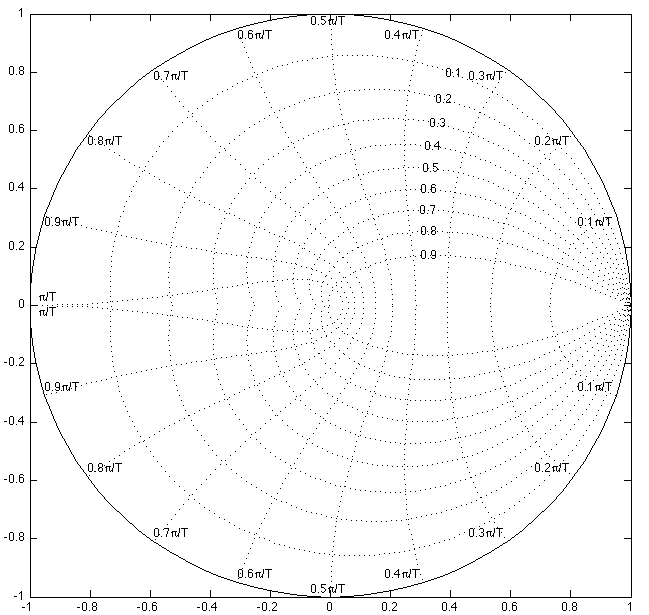
\includegraphics{pictures/zgrid.png}}
  \end{center}
\end{slide}


\section*{Continuous Design}

Assumption -- we have designed a compensator using root-locus or frequency response and now need to implement it with digital hardware, e.g. a digital micro-controller or digital signal processor (DSP).

We will recall the Discretization methods discussed in the last lecture, give a comparison of their frequency response behaviour and the applicability of the continuous design approach. We conclude with an example.

\subsection*{Discretization Procedure}

The idea is that given a continuous compensator transfer function $D(s)$ we need to find the best equivalent $D(z)$. As illustrated in \sref{slides:l12s6}, there is no exact solution since the whole time history is available to $D(s)$ whereas only samples are available to $D(z)$ so different discretization approximation methods make different assumptions about what happens to $e(t)$ between sampling instants.

\begin{slide}\label{slides:l12s6}
	\heading{Discretization Procedure}
	Given a continuous $D(s)$ find best equivalent $D(z)$.
	\begin{center}
		\resizebox{200pt}{!}{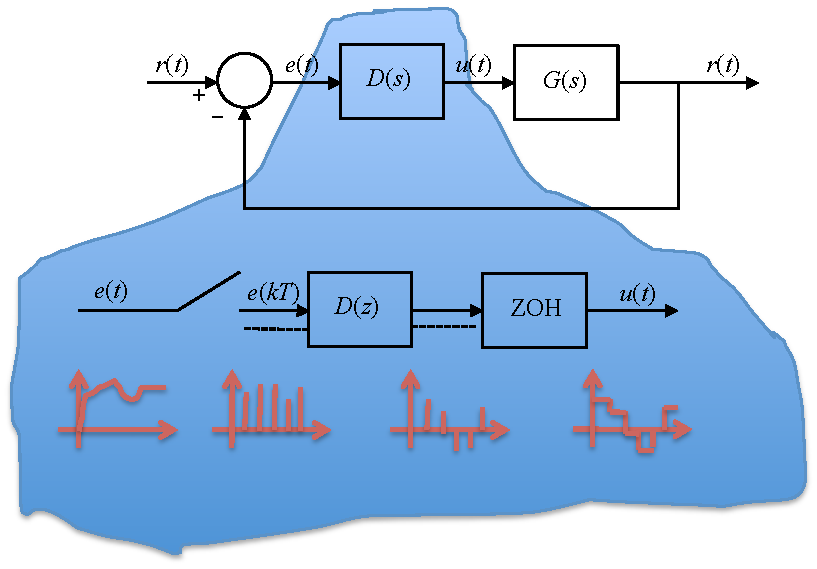
\includegraphics{pictures/digitization.pdf}}
	\end{center}
\end{slide}

\begin{slide}
	\heading{Discretization with Matlab}
	Take a transfer function (here $D(s)=p/(s+p)$) and return an equivalent $D(z)$
\begin{verbatim}
p = 5; % rad/s
ds = tf([p], [1 p])
Fs = (20*p)/(2*pi); % Hz
Ts = 1/Fs;
dz = c2d(ds, Ts, method)
step(ds,'-',dz,'--')
\end{verbatim}
\end{slide}

\begin{slide}
	\heading{Summary of Discretization Methods}
	See Lecture 11 for mathematical derivations.
	\begin{center}
		\begin{tabular}{|l|l|l|}
			\hline
			\textbf{Method} & \textbf{Transform} & \textbf{c2d method} \\
			\hline
			Zero-order hold & $(1-z^{-1})\mathcal{Z}(D(s)/s)$ & \verb|'zoh'| \\
			\hline
			Tustin (bilinear transform) & $s = (2/T)(1-z^{-1})/(1+z^{-1})$ & \verb|'tustin'| \\
			\hline
			Matched pole-zero & map poles/zeros using $z=e^{sT}$ & \verb|'matched'| \\
			\hline
			First-order hold & See Matlab documentation & \verb|'foh'| \\
			\hline
			Impulse-invariant & See Matlab documentation & \verb|'imp'| \\
			\hline
			Tustin with pre-warp & See Matlab documentation & \verb|'prewarp'| \\
			\hline
		\end{tabular}
	\end{center}
\end{slide}

\subsection*{Design Example}

Let us consider the lead compensation of the double integrator system shown in \sref{slides:ex1-1}. Let us further assume that we want to have the dominant closed-loop poles with ideal damping $\zeta=1/\sqrt{2}$ and natural frequency $\omega_n = 2\sqrt{2}$ rad/s. Furthermore, let us assume that the zero will be placed at $s=-1$ so that the compensator $D(s) = K(s+1)/(s+p)$. The root-locus design parameters will then be obtained from the pole-zero map shown in \sref{slides:ex1-2}.

$$\theta_z = \tan^{-1} 2/1 = 116.57^\circ$$

\begin{eqnarray*}
	-\theta_p + 116.57 -270 & = & -180 \\
	-\theta_p & = & -180 - 153.43 \\
	\theta_p & = & 26.57^\circ
\end{eqnarray*}

\begin{eqnarray*}
	-\tan 26.57 & = & \frac{2}{x} \\
	x & = & 2/\tan 26.57 = 4 \\
	p & = & -6
\end{eqnarray*}


\begin{slide}
	\heading{Design Example}\label{slides:ex1-1}
	\resizebox{300pt}{!}{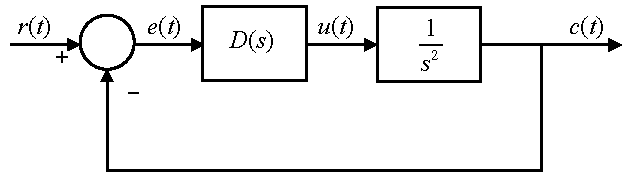
\includegraphics{pictures/ex1-1.pdf}}
\end{slide}

\begin{slide}\label{slides:ex1-2}
	\heading{Root Locus Design Parameters}
	\resizebox{300pt}{!}{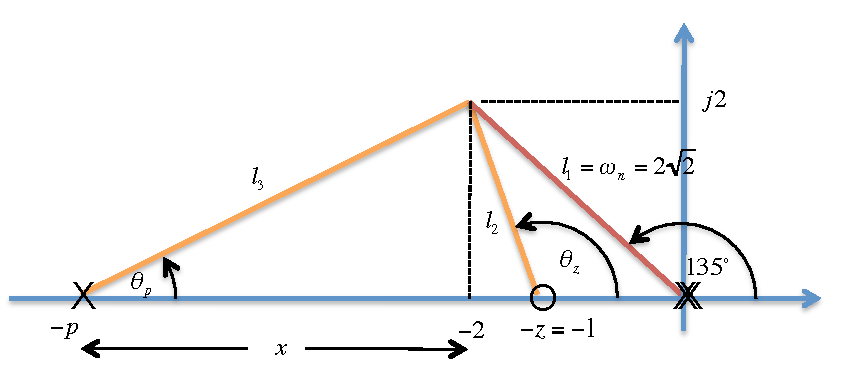
\includegraphics{pictures/ex1-2.pdf}}
\end{slide}

To calculate the gain, we need to know that $l_1=2\sqrt{2}$, $l_2=\sqrt{5}$, $l_3=\sqrt{20}$.

$$K = \frac{(2\sqrt{2})^2\times \sqrt{20}}{\sqrt{5}} = \frac{8\times 2\sqrt{5}}{\sqrt{5}} = 16.$$

$$D(s) = \frac{16(s+1)}{(s+6)}.$$

To convert to $D(z)$ let the sampling frequency $\omega_s=20\times \omega_n = 40\sqrt{2}=56.67$ rad/s. Thus $f_s=\omega_s/2\pi = 9$~Hz so sampling period $T = 1/f_s \approx 0.1$~s.

Let's pretend that we are solving this problem in a context where we only have a calculator so we'll use matched-pole zero.

$$D(z)=k\frac{1-e^{-aT}z^{-1}}{1-e^{-bT}z^{-1}}$$

where $k$ is determined by matching the DC gain of the two compensators. For the continuous compensator $D(s)|_{s=0} = 16/6$. For the digital compensator $D(z)|_{z=1} = k(1-e^{-aT})/(1-e^{-bT})$, so

$$k=\frac{16}{6}\times\frac{1-e^{-bT}}{1-e^{-aT}}$$

For our design, $T=0.1$, $a=1$ and $b=6$ so 
\begin{eqnarray*}
	k & = & \frac{16}{6}\times\frac{1-e^{-0.6}}{1-e^{-0.1}} \\
	&= & \frac{16}{6}\times\frac{1-0.5488}{1-0.9048} = \frac{16}{6}\times\frac{0.4512}{0.0952}  \\
	k & = & 12.64
\end{eqnarray*}	

So $$D(z) = \frac{12.64(1-0.9048z^{-1})}{(1-0.5488z^{-1})}$$

Since $D(z)=U(z)/E(z)$ then 
\begin{eqnarray*}
	(1-0.5488z^{-1})U(z) & = & 12.64(1-0.9048z^{-1})E(z) \\
	U(z) - 0.5488z^{-1}U(z) & = & 12.64 E(z) - 11.44 z^{-1} E(z) \\
	U(z) & = & 0.5488z^{-1}U(z) + 12.64 E(z) - 11.44 z^{-1} E(z)
\end{eqnarray*}	
Converting this into (sampled) time domain
$$u(n) = 0.5488 u(n-1) + 12.64 e(n) - 11.44 e(n-1)$$

We could implement this in pseudo code:
\begin{verbatim}
while (true) do
  /* read current error from ADC */
  e(n) = ADC 
  /* calculate and output control action */
  u(n) = 0.5488 * u(n-1) + 12.64 * e(n) - 11.44 * e(n-1)
  /* Store past values */
  e(n-1) = e(n)
  u(n-1) = u(n)
  wait for next sample time
end while
\end{verbatim}

\subsection*{Continuous Design}

\subsection*{Limits of Continuous Design Approach}

If an exact discrete analysis or a simulation of a system were performed and Discretization determined for a large range of sampling rates the digitised system would be unstable for rates slower than approximately $5\omega_n$ (where $\omega_n$ is the natural frequency of the system dominant poles) and damping would be degraded for rates slower than $10\omega_n$. At sampling rates higher than $20\omega_n$ (or $20\times \omega_{BW}$ for more complex systems) then all methods yield reasonable results and can be used with confidence at rates of $30\times \omega_{BW}$ or higher.

Errors come about because the approximations ignore the phase lag effect of the zero-order-hold (ZOH). The ZOH can be approximated by $$G_{zoh}(s)\approx \frac{2/T}{s+(2/T)}$$ which is based on the idea that, on average, the ZOH delays the signal by about $T/2$ seconds and this transfer function is a first-order lag with time constant $T/2$ and DC gain of 1. If this was added to the plant transfer function then a more accurate model of the delayed plant wiould be obtained and a more stable design for $D(s)$.

However, the advantage of continuous design is that $T$ is not chosen until after $D(s)$ is designed and the appearance of $T$ so early invalidates this assumption.

\section*{Direct Digital Design}

%----------------------------------------------------------------
% The end of notes
% ----------------------------------------------------------------
\endinput

% Local Variables:
% TeX-master: "lecture03"
% End:
